% ------------------------------------------------------------------------------
%
% PREAMBLE
%
% ------------------------------------------------------------------------------

\documentclass[12pt, titlepage]{article}


\usepackage{graphicx, amsmath, amssymb, natbib, setspace, sectsty, verbatim, 
		mathrsfs, float}
\usepackage{MnSymbol}
\usepackage{multirow}
\usepackage{bm}
\usepackage[usenames, dvipsnames]{color}
\bibpunct{(}{)}{;}{a}{}{,}
\setlength{\parindent}{3em}
%\parskip = 1.5ex
%\linespread{1.3}
%\onehalfspacing

\pdfpagewidth 8.5in
\pdfpageheight 11in
\setlength{\oddsidemargin}{0.0in} \setlength{\textwidth}{6.5in}
\setlength{\topmargin}{0.15in} \setlength{\textheight}{8.5in}
\setlength{\headheight}{0.0in} \setlength{\headsep}{0.0in}

\usepackage{/mnt/ExtraDrive1/Work/shTex/mymacros}

\providecommand{\norm}[1]{\lVert#1\rVert}
\newcommand{\csection}[1]{\section[#1]{\centering #1 }}
\subsectionfont{\small}
\newcommand{\cye}[1]{\color{yellow!70!black}#1}
\newcommand{\cre}[1]{\color{red!70!black}#1}
\newcommand{\cbl}[1]{\color{blue!70!black}#1}
\newcommand{\cgr}[1]{\color{green!70!black}#1}


% ------------------------------------------------------------------------------
%
% BEGIN DOCUMENT
%
% ------------------------------------------------------------------------------

\begin{document}

\setcounter{equation}{0}
\renewcommand{\theequation}{R.\arabic{equation}}


% ------------------------------------------------------------------------------
%
%                    Section 8.8.1
%                    Seal trend data
%
% ------------------------------------------------------------------------------

{\large \flushleft \textbf{8.8.4 Seal trend data}}

\vspace{.3cm}

Models for the harbor seal data are based on neighborhood relationships (Figure 1.3) which leads to linear models based on spatial weights (Chapter 7). In general, these types of models are amenable to fast computing because they are specified through the inverse of the covariance matrix, e.g., $\boldsymbol{\Sigma}^{-1} = \mathbf{K}_{\textrm{CAR}}^{-1}(\mathbf{I} - \rho_{\textrm{CAR}}\mathbf{W})$ (eq. 7.7 using the parsimonious models in Section 7.2).  It is the inverse of the covariance matrix that is used in the likelihoods (e.g, eqns 8.1 and 8.2), and this can be computationally demanding for large data sets if the models are specified through the covariance matrix, such as the geostatistical models (Chapter 6).  Both geostatistical and spatial-weights models also require $|\boldsymbol{\Sigma}^{-1}|$ in the likelihood, and there are special algorithms for sparse matrices such as those for the spatial-weights models.  Hence, the spatial-weights models, merely requiring an inverse of a diagonal matrix and a determinant of a sparse matrix, would seem to have a computational advantage over the geostatistical models.

However, one interesting aspect of the harbor seal example is that it contains missing data.  Ultimately, we will want to predict at these missing locations, so, for the spatial-weights models, we must include the missing locations in the neighborhood structure.  Recall that for the likelhood evaluations and optimization, we need the inverse of the covariance matrix for \textit{only} the observed data, resulting in a situation where the computational advantages of the spatial-weights models can vanish. To make this clear, let us order the locations so that all of the observed locations are first, followed by the unobserved locations, and then the covariance matrix and inverse of the covariance matrix are
\begin{equation} \label{eq:blockMats}
    \boldsymbol{\Sigma} = 
    \begin{bmatrix}
       \boldsymbol{\Sigma}_{oo} & \boldsymbol{\Sigma}_{ou} \\
       \boldsymbol{\Sigma}_{uo} & \boldsymbol{\Sigma}_{uu}
    \end{bmatrix}  \ \textrm{ and } \  
    \bSigma^{-1} = 
    \begin{bmatrix}
       \boldsymbol{\Sigma}^{oo} & \boldsymbol{\Sigma}^{ou} \\
       \boldsymbol{\Sigma}^{uo} & \boldsymbol{\Sigma}^{uu}
    \end{bmatrix}, 
\end{equation}
where the subscripts and superscripts $o$ and $u$ are for the observed and unobserved locations, respectively. The most straight-forward idea for the spatial-weights models is to obtain the covariance matrix $\boldsymbol{\Sigma}_{oo}$ by first taking $\boldsymbol{\Sigma} = (\boldsymbol{\Sigma}^{-1})^{-1}$, and then computing $\boldsymbol{\Sigma}_{oo}^{-1}$ because, unfortunately, $\boldsymbol{\Sigma}_{oo}^{-1} \neq \boldsymbol{\Sigma}^{oo}$, and, also $\boldsymbol{\Sigma}_{oo}^{-1} \neq (\boldsymbol{\Sigma}^{oo})^{-1}$. However, there is a faster way than taking the two inverses $(\boldsymbol{\Sigma}^{-1})^{-1}$ and $\boldsymbol{\Sigma}_{oo}^{-1}$, by recalling from Section 5.6 that if we already have $\boldsymbol{\Sigma}^{-1}$, then we can obtain 
$$
    \boldsymbol{\Sigma}_{oo}^{-1} = \boldsymbol{\Sigma}^{oo} - \boldsymbol{\Sigma}^{ou} (\boldsymbol{\Sigma}^{uu})^{-1} \boldsymbol{\Sigma}^{uo},
$$
which requires a single numeric inverse $(\boldsymbol{\Sigma}^{uu})^{-1}$ that has dimensions less than those of the full $(\boldsymbol{\Sigma}^{-1})^{-1}$, and will be very beneficial if the dimensions of $\boldsymbol{\Sigma}_{uu}$ are (much) less than $\boldsymbol{\Sigma}_{oo}$.  If the dimensions of $\boldsymbol{\Sigma}_{uu}$ are (much) larger than $\boldsymbol{\Sigma}_{oo}$, then the spatial-weights models, in terms of the computational demand due to matrix inverses, are more costly than geostatistical models.  For the harbor seal example, there were 306 observed locations and 157 missing locations, so we only needed a $157 \times 157$ inverse. 

We want to fit models by maximizing the log-likelihood for a variety of spatial-weights models. Figure 1.3 shows first, second, and fourth-order neighborhood relationships.  If $\mathbf{W}_{1}$ is a symmetric spatial-weights matrix as described in Chapter 7, then a matrix that includes ``neighbors of neighbors'' is
$$
\mathbf{W}_{2} = \mathcal{I}(\mathcal{I}(\mathbf{W}_{1}\mathbf{W}_{1} > 0) + \mathbf{W}_{1} > 0) - \mathbf{I}
$$
where $\mathcal{I}(\cdot)$ is the indicator function, equal to 1 if its argument is true, otherwise it is zero, and $\mathbf{I}$ is the identity matrix to ensure that the diagonal of $\mathbf{W}_{2}$ is all zeros.  In a similar fashion, we can create a fourth-order neighborhood matrix, $\mathbf{W}_{4}$ from $\mathbf{W}_{2}$.  Also, recall that for these data we have a single explanatory variable, which is a categorical (factor) variable for one of five different genetic stocks (Figure 1.1).

\begin{figure}[H]
  \begin{center}
	    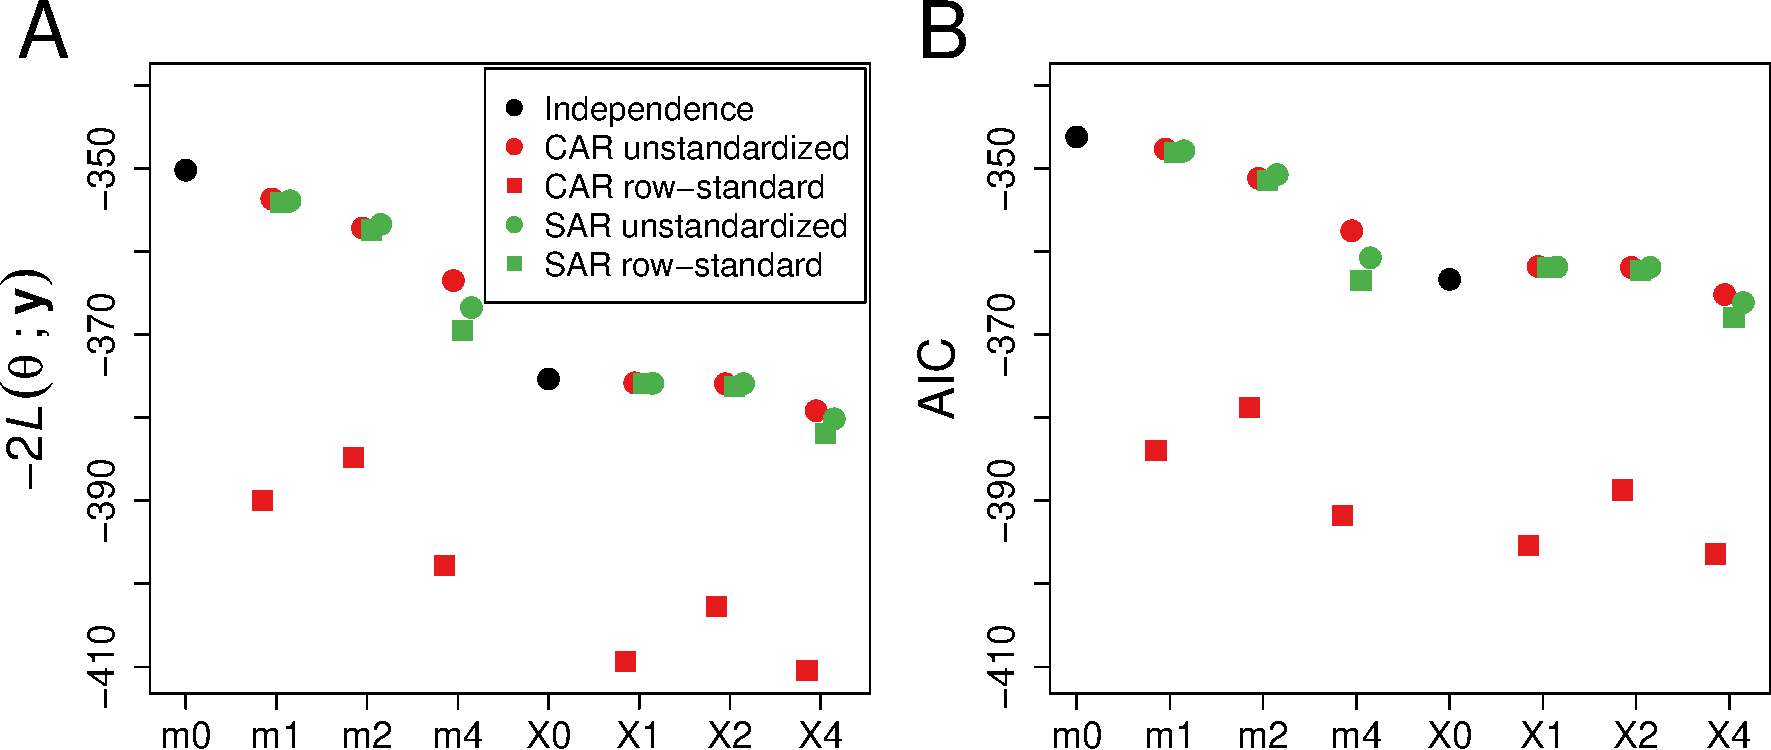
\includegraphics[width=1\linewidth]{Seals_m2LL_AIC}
  \end{center}
  \caption{Log-likelihood and AIC for a variety of spatial-weights models. A. Minus two times the log-likelihood at the ML estimate. B. AIC for the same models as given to the left.  \label{Fig:Seals_m2LLAIC}}
\end{figure}

For the harbor seal example, we want to consider a variety of models that include whether or not a spatially-autocorrelated error structure is even necessary, and if so, whether it should be a CAR or SAR model.  In both cases, we also can consider the first, second, and fourth-order neighborhood models as described above, and whether or not row-standardization was applied to those binary matrices. Figure~\ref{Fig:Seals_m2LLAIC} shows negative twice the log-likelihood, $-2L(\boldsymbol{\theta};\mathbf{y})$ (eq. 8.1), and AIC for all of these models.  Generally, we see that models including the explanatory variable fit better than those without it.  Interestingly, for the models with stock as an explanatory variable, the fits for CAR and SAR unstandardized, and SAR standardized, for first and second order neighbors were almost identical to the independence model, and so AIC favors the independence model because the spatial models have one more parameter (here, the spatial covariance can be thought of as $\boldsymbol{\Sigma} = \sigma^{2}\mathbf{R}_{\rho}$, where $\sigma^{2}$ is an overall variance parameter and $\mathbf{R}_{\rho}$ is a CAR or SAR covariance matrix that depends on the single parameter $\rho$.  The most dramatic feature of Figure~\ref{Fig:Seals_m2LLAIC} is the much improved fit when using row-standardization with the CAR models.  The best overall models suggested by AIC were the first and fourth-order, row-standardized CAR models that had stock as an explanatory variable.

Because there are only 2 covariance parameters, it is very instructive to look at the restricted log-likelihood for the variance and range parameters.  Consider the model
\begin{equation} \label{eq:seals_splm}
\mathbf(y) = \mathbf{X}\boldsymbol{\beta} + \boldsymbol{\varepsilon},
\end{equation}
where $\mathbf{X}$ contains indicator variables for genetic stock membership, and $\boldsymbol{\varepsilon}$ has a CAR covariance matrix
$$
\var(\boldsymbol{\varepsilon}) = \sigma^{2}(\mathbf{D} - \rho\mathbf{W}_{4})^{-1}
$$
where $\mathbf{D}$ is a diagonal matrix with elements $\mathbf{W}_{4}\mathbf{1}$, $\mathbf{1}$ is a vector of all ones, and recall that $\mathbf{W}_{4}$ is the fourth-order neighborhood matrix. Note that this is an equivalent way to write a CAR model with row-standardization (Section 7.3). The resulting log-likelihood surface is shown in Figure~\ref{Fig:Seals_logLik}, and the restricted maximum likelihood estimate is the value at the maximum of this surface, shown as a black circle, where $\hat{\rho} = 0.761$ and $\hat{\sigma}^{2} = 0.267$.  There are several ways to make inference on the covariance parameters, including profile likelihood and Fisher's Information matrix.

Consider the REML log-likelihood function in Section 8.2, which here is denoted as $L_{-i,R}(\theta_{i};\hat{\boldsymbol{\theta}}_{-i},\mathbf{y})$, where the $i$th component of $\boldsymbol{\theta}$ has been held constant at $\theta_{i}$, and the function has been maximized for all other parameters, whose values are denoted as $\hat{\boldsymbol{\theta}}_{-i}$.  For our model, $\boldsymbol{\theta} = (\rho, \sigma^{2})$.  Note that $\hat{\boldsymbol{\theta}}_{-i}$ changes with each $i$, but we suppress any notation to indicate such dependence. Then a profile likelihood plot for the $i$th component of $\boldsymbol{\theta}$ is one that plots $2L_{-i,R}(\theta_{i};\hat{\boldsymbol{\theta}}_{-i},\hat{\boldsymbol{\beta}},\mathbf{y})$ for various values of $\theta_{i}$, and these are seen in Figure~\ref{Fig:Seals_logLik}B for $\sigma^{2}$ and Figure~\ref{Fig:Seals_logLik}C for $\rho$.  A $1-\alpha$ level confidence interval for $\theta_{i}$ can be obtained by finding all values of $\theta_{i}$ in the profile likelihood where $2L_{-i,R}(\theta_{i};\hat{\boldsymbol{\theta}}_{-i},\mathbf{y})$ are greater than $\hat{\theta}_{i} - \chi^{2}(1-\alpha,1)$, where $\chi^{2}(x;\nu)$ is a quantile function, $0 \le x \le1$, of a chi-squared distribution on $\nu$ degrees of freedom. Using $\alpha = 0.05$ leads to a 95\% confidence interval and the well-known value of $\chi^{2}(0.95,1) = 3.841$, and $\hat{\theta}_{i} - 3.841$ are shown by the dashed lines in Figure~\ref{Fig:Seals_logLik}B,C. The confidence interval is the solid horizontal line, above which all values of $L_{-i,R}(\theta_{i};\hat{\boldsymbol{\theta}}_{-i},\hat{\boldsymbol{\beta}},\mathbf{y})$ are greater than $\hat{\theta}_{i} - 3.841$. For $\rho$, the 95\% confidence interval is from 0.347 to 0.941, and for $\sigma^{2}$, it is from 0.238 to 0.324. 

\begin{figure}[H]
  \begin{center}
	    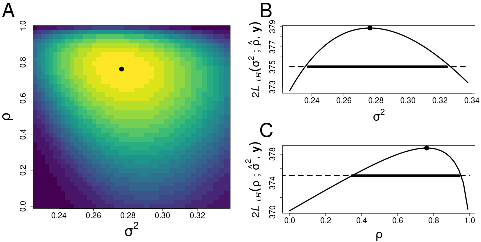
\includegraphics[width=1\linewidth]{Seals_logLik}
  \end{center}
  \caption{Restricted log-likelihood.  A. The restricted log-likelihood surface for $\rho$ and $\sigma^{2}$.  More yellow colors are higher values, and bluer colors are lower values.  The solid black circle is the maximum of the surface, yeilding the MLE. B. Profile likelihood confidence interval for $\sigma^{2}$. The curve is 2 times the restricted log-likelihood optimized for all parameters except $\sigma^{2}$, which is held constant at the value given by the x-axis.  The solid black circle is the MLE, $\hat{\sigma}^{2}$, and the dashed line is $\hat{\sigma}^{2} - \chi^{2}(1-\alpha,1)$ for $\alpha = 0.05$.  The horizontal black line forms the 95\% confidence interval.  C. Profile likelihood confidence interval for $\rho$ in the same way as described above. \label{Fig:Seals_logLik}}
\end{figure}


A second approach to finding a confidence interval is based on large sample asymptotics, where the curvature of the likelihood in Figure~\ref{Fig:Seals_logLik} at the REMLE (or we could also use MLE) is approximated by the observed Fisher's Information matrix, which can be used to construct confidence intervals as suggested in Section 8.4.  After fitting the model, we compute observed Fisher's Information,
$$
\boldsymbol{J}_{a}{(\boldsymbol{\theta})_{i,j}} = \frac{1}{2}\operatorname{tr}\left(\boldsymbol{\Sigma}^{-1} \frac{\partial \boldsymbol{\Sigma}}{\partial\theta_i}{\boldsymbol{\Sigma}^{-1}}\frac{\partial\boldsymbol{\Sigma}}{\partial\theta_j}\right),
$$
by using $\boldsymbol{\Sigma}^{-1} = (\mathbf{D} - \hat{\rho}\mathbf{W})/\hat{\sigma}^{2}$ and noting that 

\begin{align*}
	\frac{\partial \boldsymbol{\Sigma}}{\partial\sigma^{2}} = & (\mathbf{D} - \rho\mathbf{W}_{4})^{-1}, \\
	\frac{\partial \boldsymbol{\Sigma}}{\partial\rho} = & \sigma^{2}(\mathbf{D} - \rho\mathbf{W}_{4})^{-1}\mathbf{W}_{4}(\mathbf{D} - \rho\mathbf{W}_{4})^{-1},
\end{align*}
where $\sigma^{2}$ and $\rho$ are replaced by $\hat{\sigma}^{2}$ and $\hat{\rho}$, respectively. 

An estimator of the asymptotic standard errors of $\hat{\boldsymbol{\theta}}$ are the square roots of the diagonal of $[\boldsymbol{J}_{a}{(\boldsymbol{\theta})}]^{-1}$.  Formally, let $\mathbf{j}_{i}$ be a vector of all zeros, except there a single one at the $i$th element.  Then a $(1 - \alpha)100$\% confidence interval for $\hat{\theta}_{i}$ is
$$
\hat{\theta}_{i} \pm z_{1-\alpha/2}\sqrt{\mathbf{j}_{i}^{T}[\boldsymbol{J}_{a}{(\boldsymbol{\theta})}]^{-1}\mathbf{j}_{i}},
$$
where $z_{1-\alpha/2}$ is a quantile of a standard normal distribution at $1-\alpha/2$.  For example, if $\alpha = 0.05$, then $z_{1-\alpha/2}$ is the familiar 1.96.  In our example, the standard errors for $\rho$ and $\sigma^{2}$ were 0.101 and 0.018, respectively, so the 95\% confidence interval for $\rho$ was from 0.563 to 0.959 and for $\sigma^{2}$ it was from 0.240 to 0.312, which can be compared to those obtained from profile likelihood.

Another approach is to compute the Hessian matrix of the log-likelihood.  We used \texttt{spmodel} for this as it allowed us to evaluate the log-likelihood for any given value of $\boldsymbol{\theta}$.  We used the \texttt{R} package \texttt{numDeriv} to compute the numeric Hessian, $\mathbf{H}$, at the REMLE, and then an estimator of Fisher's Information is,
$$
\boldsymbol{J}_{n}{(\boldsymbol{\theta})} = -\mathbf{H},
$$
and an estimator of the asymptotic standard errors follow in exactly the same way as they were developed when using $\boldsymbol{J}_{a}{(\boldsymbol{\theta})}$.  In our example, the standard errors for $\rho$ and $\sigma^{2}$ were 0.145 and 0.023, respectively, so the 95\% confidence interval for $\rho$ was from 0.476 to 1.046 and for $\sigma^{2}$ it was from 0.231 to 0.321, which can be compared to those obtained from the analytical computation of Fisher's Information and profile likelihood.  Here, the confidence interval for $\rho$ extends beyond 1 at the upper bound, showing a disadvantage of the large-sample asymptotic approach that relies on normality.

Nevertheless, it is interesting to look at the asymptotic correlation among the parameters as revealed by the observed Fisher's Information matrix.  Let $\mathbf{S}_{a}$ be a diagonal matrix containing reciprocals of the square roots from the diagonal of $[\boldsymbol{J}_{a}{(\boldsymbol{\theta})}]^{-1}$, and similarly obtain $\mathbf{S}_{n}$ from $[\boldsymbol{J}_{n}{(\boldsymbol{\theta})}]^{-1}$ .  Then estimators of the asymptotic correlation matrix are
$$
\mathbf{S}_{a}[\boldsymbol{J}_{a}{(\boldsymbol{\theta})}]^{-1}\mathbf{S}_{a} =
\left(
\begin{array}{rr}
1.000 & 0.163 \\ 
  0.163 & 1.000  \\ 
\end{array}
\right) \textrm{ and }
\mathbf{S}_{n}[\boldsymbol{J}_{n}{(\boldsymbol{\theta})}]^{-1}\mathbf{S}_{n} =
\left(
\begin{array}{rr}
1.000 & -0.189 \\ 
  -0.189 & 1.000  \\ 
\end{array}
\right),
$$
which show little correlation between $\rho$ and $\sigma^{2}$, and this is also evident in the shape of the log-likelihood surface (Figure~\ref{Fig:Seals_logLik}A).
 
One of the features of the spatial-weights models is that they are nonstationary, and it is interesting to investigate this property for actual data.  First, consider two models as in \eqref{eq:seals_splm}, using the fourth-order neighborhood structure, one where the $\mathbf{W}$ is standardized, i.e., $\var(\boldsymbol{\varepsilon}) = \boldsymbol{\Sigma}_{rs} = \sigma^{2}_{rs}(\mathbf{I} - \rho_{rs}\overline{\mathbf{W}}_{4})\mathbf{K}_{rs}$, and the other where it is not, i.e., $\var(\boldsymbol{\varepsilon}) = \boldsymbol{\Sigma}_{un} = \sigma^{2}_{un}(\mathbf{I} - \rho_{un}\mathbf{W}_{4})\mathbf{K}_{un}$. The diagonal elements of $\boldsymbol{\Sigma}_{rs}$, plotted as a function of the number of neighbors, is shown in Figure~\ref{Fig:seals_nonstationary}A.  Notice that the marginal variance goes down with increasing numbers of neighbors.  This is reasonable because, recall from eq. 7.6, the $c_{ij}$ weights are 1/(number of neighbors) when they are row standardized, so we are \textit{averaging} over neighboring values, and the variance of an average goes down with larger sample sizes.  On the other hand, the marginal variances of $\boldsymbol{\Sigma}_{un}$ are shown in Figure~\ref{Fig:seals_nonstationary}B, where $c_{ij} = 1$ in (7.6) so we are \textit{summing} over neighboring values, and the variance of a sum goes up with larger sample sizes.  Moreover, even for a fixed number of neighbors, the variance is not constant because (7.6) specifies a conditional expectation and the marginal variances involve the inverse of the matrix specified by these weights. In summary, both of these models exhibit nonstationary variances, in contrast to geostatistical models, where variances are constant regardless of distance.

Similarly, we can look at autocorrelation as a function of the order of the neighbor. Let $\mathcal{N}_{i}^{[1]}$ be the set of all neighbors of site $i$, $\mathcal{N}_{i}^{[2]}$ be the set of all neighbors of $\mathcal{N}_{i}^{[1]}$, exclusive of any already in $\mathcal{N}_{i}^{[1]}$, $\mathcal{N}_{i}^{[3]}$ be the set of all neighbors of $\mathcal{N}_{i}^{[2]}$, exclusive of any already in $\mathcal{N}_{i}^{[1]}$ or $\mathcal{N}_{i}^{[2]}$, etc., up to sixth-order neighbors.  Then pairwise autocorrelations taken from $\boldsymbol{\Sigma}_{rs}$, as a function of neighbor order, are plotted as violin plots in Figure~\ref{Fig:seals_nonstationary}C.  In general autocorrelation decreases as a function of neighbor order, but there is wide variation for a given neighbor order.  It is also interesting to see that for the fourth-order neighbor model that was fit, there is a sudden decrease in autocorrelation, on average, after order four. Nonetheless, Figure~\ref{Fig:seals_nonstationary}C also shows that autocorrelation exists in $\boldsymbol{\Sigma}_{rs}$ beyond fourth order, even though $\overline{\mathbf{W}}_{4}$ contains all zeros beyond fourth order.  Like variances, this is due to the fact that $\boldsymbol{\Sigma}_{rs}$ is obtained through an inverse involving $\overline{\mathbf{W}}_{4}$, rather than $\overline{\mathbf{W}}_{4}$ directly.
 \begin{figure}[H]
  \begin{center}
	    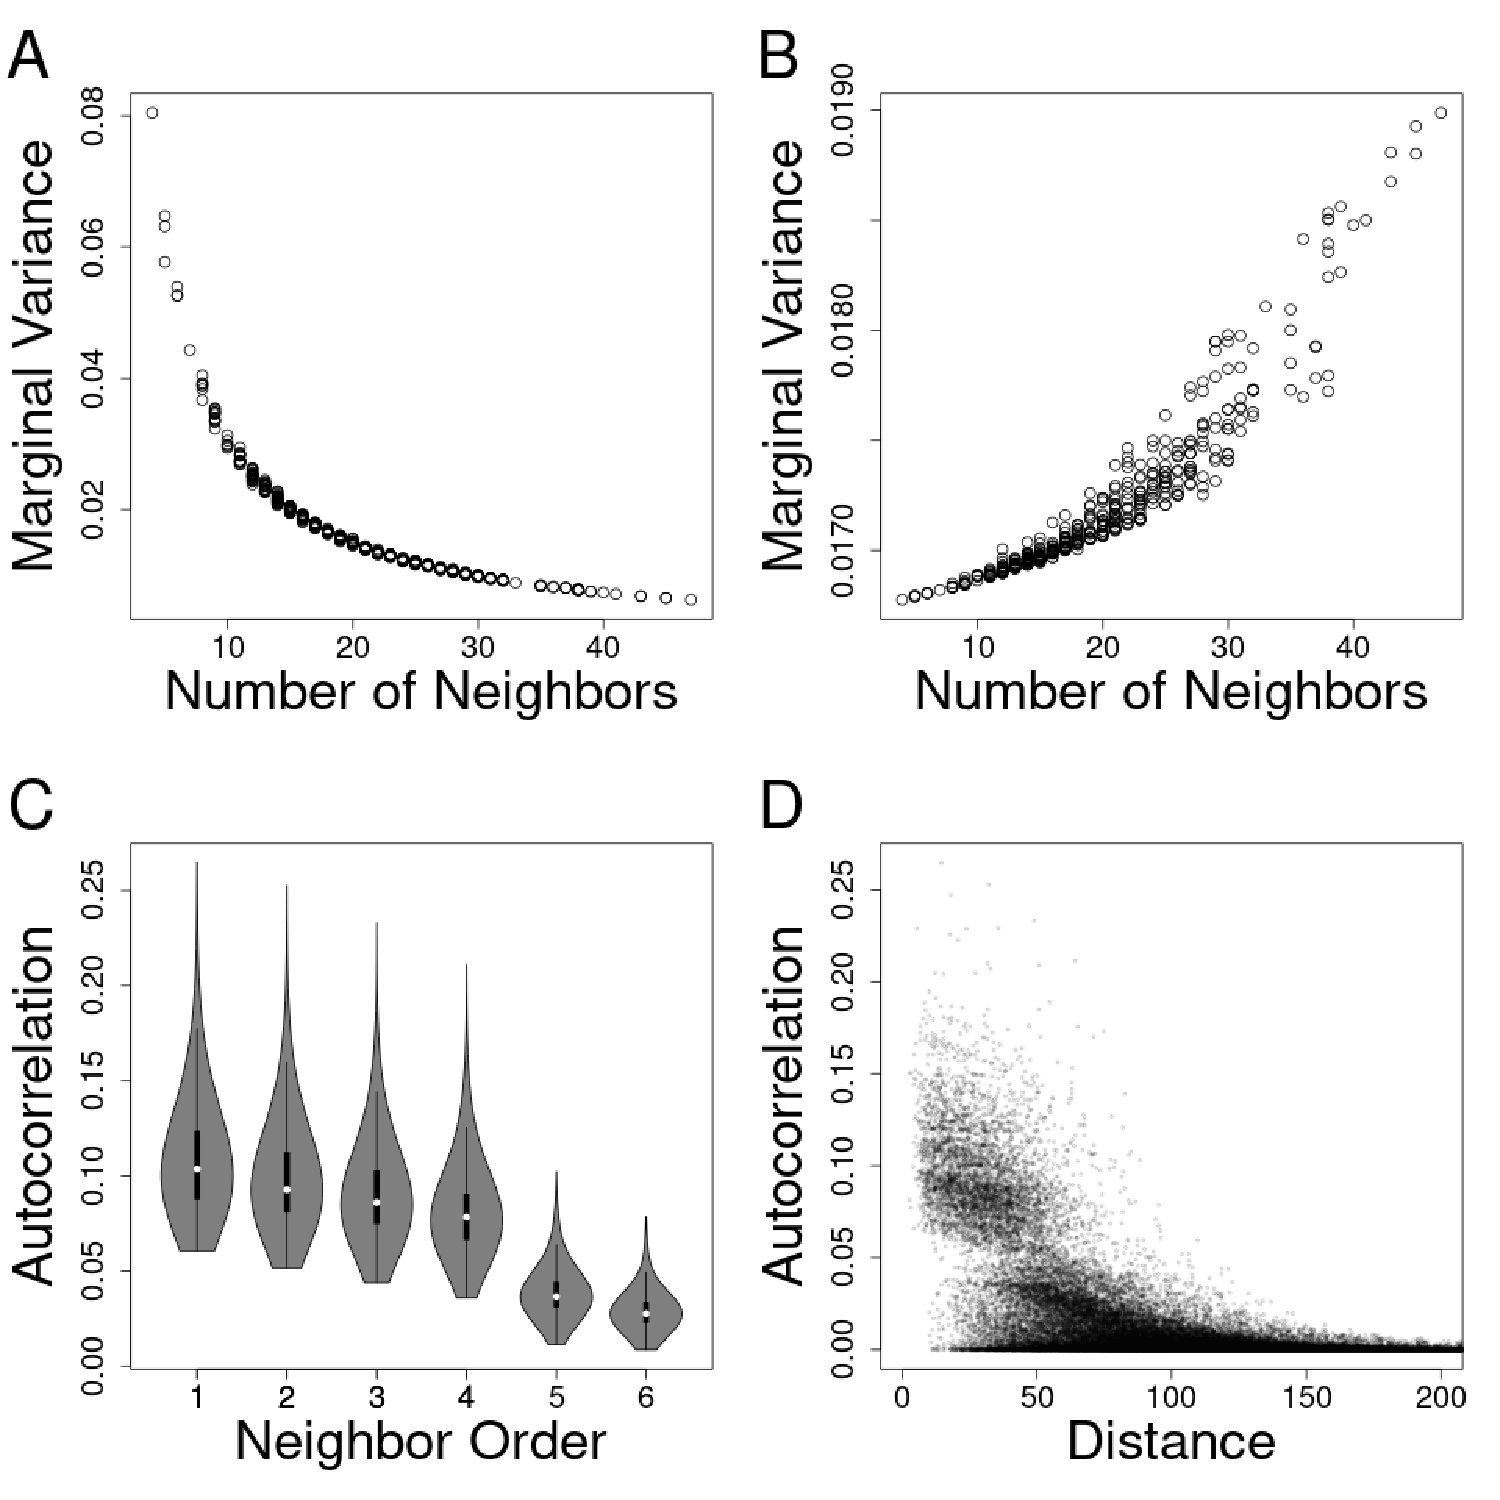
\includegraphics[width=.8\linewidth]{Seals_nonstationary}
  \end{center}
  \caption{Nonstationarity in spatial-weights models. A. Marginal variance as a function of number of neighbors for a row-standardized CAR model. B. Marginal variance as a function of number of neighbors a binary weights CAR model. C. Violin plots of autocorrelation as a function of neighbor order for row-standardized cAR model. D. Scatterplot of all pairwise correlations as a function of centroid distance for row-standardized CAR model. \label{Fig:seals_nonstationary}}
\end{figure}

Although distance is not often well-defined for the spatial-weights models, such as when sites are polygons as in this harbor seals example, one unique definition of distance is obtained by associating a centroid with each polygon, and then taking Euclidean distances among centroids.  Plotting autocorrelation as a function of centroid distance shows that, in general, autocorrelation decreases with distance (Figure~\ref{Fig:seals_nonstationary}D), just as it did for neighbor order (\ref{Fig:seals_nonstationary}C).  Again, compare this situation to an isotropic geostatistical model, where autocorrelation is fixed for any given distance between two locations.

Before moving to estimation of fixed effects, we consider a few more models.  One very handy feature of the \texttt{spmodel} software is that it allows the estimation of a separate variance parameter for sites that are isolated, as discussed in Section 7.4.  By default, the software uses the geometry in \texttt{sf} objects and determines neighbors as any polygons that share a common boundary.  Fitting a CAR model in this way, including the genetic stock explanatory variable, and ordering the data so that the isolated polygons are listed first, the ML estimated covariance matrix for the row-standardized model was
$$
\boldsymbol{\Sigma}(\hat{\boldsymbol{\theta}}) = \left({}
	\begin{array}{cc}
	  0.043\times\mathbf{I} & \mathbf{0} \\
	  \mathbf{0} & 0.032\times(\mathbf{I} - 0.264\times\overline{\mathbf{W}})^{-1}\overline{\mathbf{K}}
	\end{array}
\right),
$$
and $-2L(\boldsymbol{\theta},\mathbf{y}) = -418.99$.  With five fixed effects and three covariance parameters, AIC = -402.99, and, even though it has an extra covariance parameter, it is the best model when compared to all of those in Figure~\ref{Fig:Seals_m2LLAIC}.  Geostatistical models are stationary, and the centroids can be used as distance between polygons.  Using distance in this way, the best geostatistical model with the explanatory variable, using MLE, was a circular model, which had $-2L(\boldsymbol{\theta},\mathbf{y}) = -390.66$, and, again with three covariance parameters, AIC was -374.66, which was considerably worse than the row-standardized CAR model with islands.  Finally, the variance-stabilizing weights of Section 7.3 were used in a CAR model (without islands) and with the explanatory variable, yielding $-2L(\boldsymbol{\theta},\mathbf{y}) = -399.93$, and, with two covariance parameters, AIC was -385.93.

Any choice of a covariance model, and fitting it, leads to the next topic -- inference about the fixed effects -- which was broadly covered in Chapter 5.  Let $\boldsymbol{\Sigma}(\hat{\boldsymbol{\theta}})$ be estimated by ML using a row-standardized CAR model with islands, as described in the previous paragraph, with a mean structure that includes an overall intercept and genetic stock membership as a categorical explanatory variable, as this appeared to be the best model according to AIC. Then an empirical \textit{GLS} estimate of stock effect $\tilde{\tilde{\boldsymbol{\beta}}} = [\mathbf{X}^{T}[\boldsymbol{\Sigma}(\hat{\boldsymbol{\theta}})]^{-1}\mathbf{X}]^{-1}\mathbf{X}^{T}(\boldsymbol{\Sigma}(\hat{\boldsymbol{\theta}}))^{-1}\mathbf{y}$ is given in Table~\ref{tab:stockFE} in typical \texttt{R} format, where $\tilde{\tilde{\boldsymbol{\beta}}}$ is given in the column labeled as ``Estimate.''
\begin{table}[H] 
	\caption{Coefficient table of fixed effects estimated by ML using a row-standardized CAR model with islands, as given by the \texttt{spmodel} package in \texttt{R}.  The first column is the estimated coefficients of $\tilde{\tilde{\boldsymbol{\beta}}}$, the second column is the estimated standard error, the third column is a computed z-value where column 1 is divided by column two, and the fourth column is the estimated probability of obtaining the z-value if the null hypothesis that the effect was zero was true.  \label{tab:stockFE}}
\begin{center}
\begin{tabular}{|c|rrrr|}
  \hline
  \hline{}
  Coefficients & Estimate & Std. Error & z-value & Pr($>|z|$) \\
	\hline
  \hline
(Intercept) & 0.0069 & 0.0127 & 0.547 & 0.58435 \\ 
  stock Dixon/Cape Decision & 0.0449 & 0.0200 & 2.249 & 0.02453 \\ 
  stock Glacier Bay/Icy Strait & -0.0785 & 0.0265 & -2.970 & 0.00298 \\ 
  stock Lynn Canal/Stephens & -0.0334 & 0.0242 & -1.381 & 0.16743 \\ 
  stock Sitka/Chatham & 0.0129 & 0.0211 & 0.613 & 0.53999 \\ 
  \hline
  \hline
\end{tabular}
\end{center}
\end{table}

Standard errors for $\tilde{\tilde{\beta}}_{i}$, the $i$th element of $\tilde{\tilde{\boldsymbol{\beta}}}$, are estimated as  $\tilde{\tilde{\sigma}}_{i} = \sqrt{[\mathbf{X}^{T}[\boldsymbol{\Sigma}(\hat{\boldsymbol{\theta}})]^{-1}\mathbf{X}]^{-1}_{i,i}}$.  As discussed in Section 5.7, distributional properties of the empirical generalized least squares are complicated due to the fact that, from (8.3), $\boldsymbol{\Sigma}(\hat{\boldsymbol{\theta}}) = \tilde{\tilde{\sigma}}^{2}\mathbf{R}(\hat{\boldsymbol{\theta}}_{-1})$.  Nevertheless, assuming that $\tilde{\tilde{\boldsymbol{\beta}}}$ is approximately normal, a $z$-value can be formed as $\tilde{\tilde{\beta}}_{i}/\tilde{\tilde{\sigma}}_{i}$, the third column in Table~\ref{tab:stockFE}. Let $z$ have a standard normal distribution with cumulative distribution function $\boldsymbol{\Phi}(z)$. Then an approximate $\alpha$-level test against the null hypothesis that $\tilde{\tilde{\beta}}_{i} = 0$ is given by the probability of obtaining the computed z-value, or larger, Prob($|\tilde{\tilde{\beta}}_{i}/\tilde{\tilde{\sigma}}_{i,i}| > z)$, so $\alpha = 2\times(1 - \boldsymbol{\Phi}(|\tilde{\tilde{\beta}}_{i}/\tilde{\tilde{\sigma}}_{i}|))$, which is the fourth column in Table~\ref{tab:stockFE}.

It is also possible to pivot on the estimated $z$-value to obtain confidence intervals using the inverse cumulative distribution function, also called a quantile function, $\boldsymbol{\Phi}^{-1}(p)$. Let $z_{1-\alpha/2} = \boldsymbol{\Phi}^{-1}(1-\alpha/2)$, then a $(1-\alpha/2)\times100\%$ confidence interval for $\tilde{\tilde{\beta}}_{i}$ is $\tilde{\tilde{\beta}}_{i} \pm z_{1-\alpha/2}\tilde{\tilde{\sigma}}_{i}$.  For example, recall that the stock effect for ``Clarence Strait'' has been absorbed into the overall intercept, so that the effect ``Dixon/Cape Decision'' is an estimate of the \textit{difference} between Clarence Strait and Dixon/Cape Decision.  A 95\% confidence interval on this difference is $0.449 \pm 1.96 \times 0.02 = (0.0057, 0.0841)$. If an estimate of Dixon/Cape Decision is desired, then let $\boldsymbol{\ell}$ be the vector $(1, 1, 0, 0, 0)$, and then the estimator of the Dixon/Cape Decision effect is $\boldsymbol{\ell}^{T}\tilde{\tilde{\boldsymbol{\beta}}}$, which for our example is 0.0518, with standard error $\sqrt{\boldsymbol{\ell}^{T}[\mathbf{X}^{T}(\boldsymbol{\Sigma}(\hat{\boldsymbol{\theta}}))^{-1}\mathbf{X}]^{-1}\boldsymbol{\ell}}$, which for our example is 0.0155.  Then a 95\% confidence interval for the log-trend of the  Dixon/Cape Decision stock is 0.0215 to 0.0821, and we can be 95\% certain that the stock is growing from somewhere between approximately 2\% to 8\% per year.  In addition to estimates, we are often interested in specific contrasts. Figure~1.1 shows stocks labelled 8 and 9 as the two northern stocks, while stocks 10, 11, and 12 are southerns stocks.  We would like to estimate the difference in trends between the northern and southern stocks.  Stock 8 is Glacier Bay/Icy Strait, and stock 9 is Lynn Canal/Stephens, so the contrast of interest is $[\beta_{1} + (\beta_{2} + \beta_{1}) + (\beta_{5} + \beta_{1})]/3 - [(\beta_{3} + \beta_{1}) + (\beta_{4} + \beta_{1})]/2$ = $\boldsymbol{\ell}^{T}\tilde{\tilde{\boldsymbol{\beta}}}$, where $\boldsymbol{\ell} = (0, 1/3, -1/2, -1/2, 1/3)$. The estimate of this contrast is 0.0752, with standard error of 0.0177, and a 95\% confidence interval difference in log-trend of the difference between the northern and southern stocks ranges from 0.0404 to 0.1101, and we can be 95\% certain that the southern stocks trends are somewhere between approximately 4\% to 11\% higher per year than the northern stocks.

In addition to estimating individual effects, their linear combination, or a contrast, interest often centers on whether the stock effect as a whole should be included in the model.  Chapter 5 developed an $F$-test for a joint linear hypothesis $\mathbf{L}\hat{\boldsymbol{\beta}} = \mathbf{0}$, where $\mathbf{0}$ is a vector of all zeros, in the case where $\mathbf{R}$ is known.  The numerator of that $F$-test is distributed as a chi-squared random variable, which the \texttt{spmodel} package uses  in the $EGLS$ situation as an approximation to the distribution of $\mathbf{L}\tilde{\tilde{\boldsymbol{\beta}}}$.  Specifically, let $\mathbf{L}$ be the matrix $(\mathbf{0}_{4}|\mathbf{I}_{4})$ where $\mathbf{0}_{4}$ is a vector of four zeros and $\mathbf{I}_{4}$ is the $4 \times 4$ identity matrix.  Then, for our example,
$$
X = (\mathbf{L}\tilde{\tilde{\boldsymbol{\beta}}})^{T}
[\mathbf{L}\mathbf{X}^{T}(\boldsymbol{\Sigma}(\hat{\boldsymbol{\theta}}))^{-1}\mathbf{X}\mathbf{L}^{T}]^{-1}\mathbf{L}\tilde{\tilde{\boldsymbol{\beta}}} = 23.0895
$$
and if $F_{\chi^{2}}(x,\nu)$ is the cumulative distribution function for a chi-squared random variable with $\nu$ degrees of freedom, then = $1 - F_{\chi^{2}}(23.0895,4) = 0.000122$ is the probability of obtaining the observed value, or larger, if the null hypothesis were true.  These results are obtained with the \texttt{anova} function in \texttt{spmodel}.

An alternative way to determine the effect of genetic stock, after accounting for the overall mean effect, is by a likelihood ratio test, which is very general.  Recall that $-2L(\boldsymbol{\theta};y,\mathbf{X}_{\textrm{stock}}) = -418.99$ for the model with stock as an explanatory variable, and allowing for isolated sites and a row-standardized CAR model. Using a mean-only model with the same covariance structure results in $-2L(\boldsymbol{\theta};y,\mathbf{X}_{\textrm{ones}}) = -398.74$. The difference in these two log-likelihoods is 20.2427, and under large-sample aymptotics this has a chi-squared distribution, so  $1 - F_{\chi^{2}}(20.2427,4) = 0.000447$ and the probability of obtaining the observed value, or larger, if the mean-only model were true.  These results can also be obtained with the \texttt{anova} function in \texttt{spmodel}.


%%%%%%%%%%%%%%%%%%%%%%%%%%%%%%%%%%%%%%%%%%%%%%%%%%%%%%%%%%%%%%%%%%%%%%%%%%%%%%%%
%%%%%%%%%%%%%%%%%%%%%%%%%%%%%%%%%%%%%%%%%%%%%%%%%%%%%%%%%%%%%%%%%%%%%%%%%%%%%%%%                BIBLIOGRAPHY
%%%%%%%%%%%%%%%%%%%%%%%%%%%%%%%%%%%%%%%%%%%%%%%%%%%%%%%%%%%%%%%%%%%%%%%%%%%%%%%%
%%%%%%%%%%%%%%%%%%%%%%%%%%%%%%%%%%%%%%%%%%%%%%%%%%%%%%%%%%%%%%%%%%%%%%%%%%%%%%%%

%\bibliographystyle{consbiol}
\bibliographystyle{/mnt/ExtraDrive1/Work/shTex/asa}
\bibliography{DaleChap883.bib}
%\bibliographystyle{/home/jay/Data/shTex/shTex/asa}
%\bibliography{/home/jay/Data/shTex/shTex/StatBibTex.bib}




\end{document}

